\documentclass{article}
\usepackage{amsfonts}
\usepackage{amsmath}
\usepackage{graphicx} 
\usepackage{hyperref}
\usepackage[parfill]{parskip}
\usepackage{float}

\title{Abgabe 1 für Computergestütze Methoden}
\author{Gruppe 37, Arman Avetisyan (4265195), Berkay Okkuscu (4251181)}
\date{02.12.2024}

\begin{document}

\maketitle
\renewcommand{\contentsname}{Inhaltsverzeichnis}
\tableofcontents
\newpage
\section{Der zentrale Grenzwertsatz} 
     Der zentrale Grenzwertsatz (ZGS) ist ein fundamentales Resultat der Wahrscheinlichkeitstheorie, das die Verteilung von Summen unabhängiger, identisch verteilter $(i.i.d.)$ Zufallsvariablen (ZV) beschreibt. Er besagt, dass unter bestimmten Voraussetzungen die Summe einer großen Anzahl solcher ZV annähernd normalverteilt ist, unabhängig von der Verteilung der einzelnen ZV. Dies ist besonders nützlich, da die Normalverteilung gut untersucht und mathematisch handhabbar ist.


\subsection{Aussage}
    Sei $X_1,X_2,...,X_n$ eine Folge von $i.i.d.$ ZV mit dem Erwartungswert $\mu=\mathbb{E}(X_i)$ und der Varianz $\sigma^2$ = Var($X_i$), wobei $0 < \sigma^2 < \infty$ gelte. Dann konvergiert die standardisierte Summe $Z_n$ dieser ZV für $n \rightarrow \infty$ in Verteilung gegen eine Standardnormalverteilung:\footnote[1]{Der zentrale Grenzwertsatz hat verschiedene Verallgemeinerungen. Eine davon ist der \textbf{Lindeberg-Feller-Zentrale-Grenzwertsatz} [\cite{klenke2013}, Seite 328], der schwächere Bedingungen an die Unabhängigkeit und die identische Verteilung der ZV stellt.}
    \begin{equation}
        \label{Summe}
        Z_n = \frac{\sum_{i = 1}^nX_i-n\mu}{\sigma\sqrt{n}} \rightarrow \mathcal{N}(0,1)
    \end{equation}
    Das bedeutet, dass für große $n$ die Summe der ZV nährungsweise normalverteilt ist mit dem Erwartungswert $n\mu$ und Varianz $n\sigma^2$:
    \begin{equation}
    \label{Summe2}
        \sum_{i=1}^nX_i\sim\mathcal{N}(n\mu, n\sigma^2)
    \end{equation}


\subsection{Erklärung der Standardisierung}
    Um die Summe der ZV in eine Standardnormalverteilung zu transformieren, subrtrahiert man den Erwartungswert $n\mu$ und teilt durch die Standardabweichung $\sigma\sqrt{n}$. Dies führt zu der obigen Formel \eqref{Summe}. Die Darstellung \eqref{Summe2} ist für $n \rightarrow \infty$ nicht wohldefiniert.

    
\subsection{Anwendung}
Der ZGS wird in vielen Bereichen der Statistik und der Wahrscheinlichkeitstheorie angewendet. Typische Beispiele:
\begin{itemize}
\item Zwei Würfel werdem $n$ Mal geworfen. Augensumme von 2-12 möglich. Einzelnen Augensummen $i.i.d$ verteilt. 36 mögliche Würfelkonstelationen, häufigste die 7. Durch ZGS die Augensumme von $n$-Würfen normalverteilt.

\begin{equation}
\Bar{X_n}\sim\mathcal{N}(\mu,\frac{\sigma^2}{n})
\end{equation}
\item Ein Hersteller für Schrauben möchte wissen, ob die Maschine korrekt arbeitet, indem er den Durchschnitt der Längen aus einer Stichprobe von 50 Schrauben misst.
Nach dem ZGS ist der Stichprobenmittlewert $\Bar{X}$ für $n = 50$ nährungsweise normalverteilt:
\begin{equation}
    \Bar{X}\sim\mathcal{N}(\mu,\frac{\sigma^2}{n}) = \mathcal{N}(10,\frac{0.2^2}{50})
\end{equation}
\end{itemize}




\section{Bearbeitung zur Aufgabe 1}
\subsection{Datenverarbeitung}

\subsubsection{Untersuchung der Relevanten Daten}
Die erste Beobachtung ist, dass der Datensatz als ein CSV-Dokument gegeben ist. Der von Gruppe 37 zugeordnete Datenteil ist "Cleveland Pl \& Spring St". 
Die Daten die angezeigt wurden, waren das Datum, der wievielte Tag des Jahres, der wievielte Tag der Woche, der Monat, der Niederschlag, Windgeschwindigkeit, 
die Mindest- Durschnitts- und Höchsttemperatur und die Anzahl der ausgeliehenen Fahrräder.

Die Attributnamen werden in der obersten Zeile aufgeführt und die dazugehörigen Attribute werden darunter aufgelistet, um einen einfacheren Überblick zu verschaffen.

Nun wurde der Datensatz in die Tabellenkalkulation importiert, damit im dazugehörigen Datenteil von Gruppe 37 die höchste durchschnittliche Temperatur in Grad Celsius berechnet werden kann. Mit der Tabellenkalkulation kann man die Daten z.B. nach der Gruppe filtern.

\subsubsection{Höchsten durchschnittlichen Temperatur in Grad Celsius}
Die Nutzung der Filterfunktion war der erste Schritt, um für unsere Gruppe den zugehörigen Datenteil anzeigen zu lassen.

Danach wurde die Spalte \textit{mean\_temperature} von der höchsten zur niedrigsten Temperatur sortiert um die höchste Temperatur in Fahrenheit herauszufinden. Um die höchste mittlere Durchschnittstemperatur in Celsius umzurechnen wurde der Befehl \textit{UMRECHNEN} genutzt.

In Fahrenheit betrug die höchste mittlere Durchschnittstemperatur $83^\circ\text{F}$. In Celsius waren es $28^\circ\text{C}$.


\newpage

\subsection{Datenhaltung}
Erklärung des SQL-Codes:

Der SQL-Code definiert zunächst eine Tabelle namens \textit{weather\_data}, die Wetterdaten systematisch speichert. Die Anweisung \textit{CREATE TABLE IF NOT EXIST} verhindert, dass die Tabelle bei mehrfacher Ausführung erneut erstellt wird. Die Tabelle enthält folgende Spalten:


\begin{itemize}
    \item \textit{station} und \textit{date} speichern die Wetterstation und das Datum der Beobachtung (beide \textit{NOT NULL}) 
    \item \textit{day\_of\_year}, \textit{day\_of\_weak} und \textit{month\_of\_year} dienen der zeitlichen Einordnung der Daten 
    \item \textit{precipton} und \textit{windspeed} erfassen Niederschlagsmengen und Windgeschwindigkeiten
    \item \textit{min\_temperature}, \textit{average\_temperature}, \textit{max\_temperature} und \textit{average\_temperature\_celsius speichern} Temperaturwerte
    \item Zählung steht für die Anzahl der geliehenen Fahrräder an dem dazugehörigen Tag
\end{itemize}

Nach der Tabellendefinition werden mittels \textit{INSERT INTO} (\ref{Abb1}) \& (\ref{Abb2}) eine Vielzahl von Datensätzen eingefügt, die detaillierte Wetterbeobachtungen wie Datum, Temperatur und Windgeschwindigkeit enthalten.

Die abschließenden Abfragen, \textit{SELECT*FROM weather\_data} und \textit{PRAGMA  table\_info(weather\_data)} (\ref{Abb2}), dienen der Anzeige der gespeicherten Daten und der Tabellenspezifikationen.

\textbf{Fazit:} Dieser Code ermöglicht eine strukturierte Speicherung und spätere Analyse von Wetterdaten. Die gewählte Tabellenstruktur bietet Flexibilität für Abfragen und Auswertungen. 



\begin{figure}[p]
    \centering
    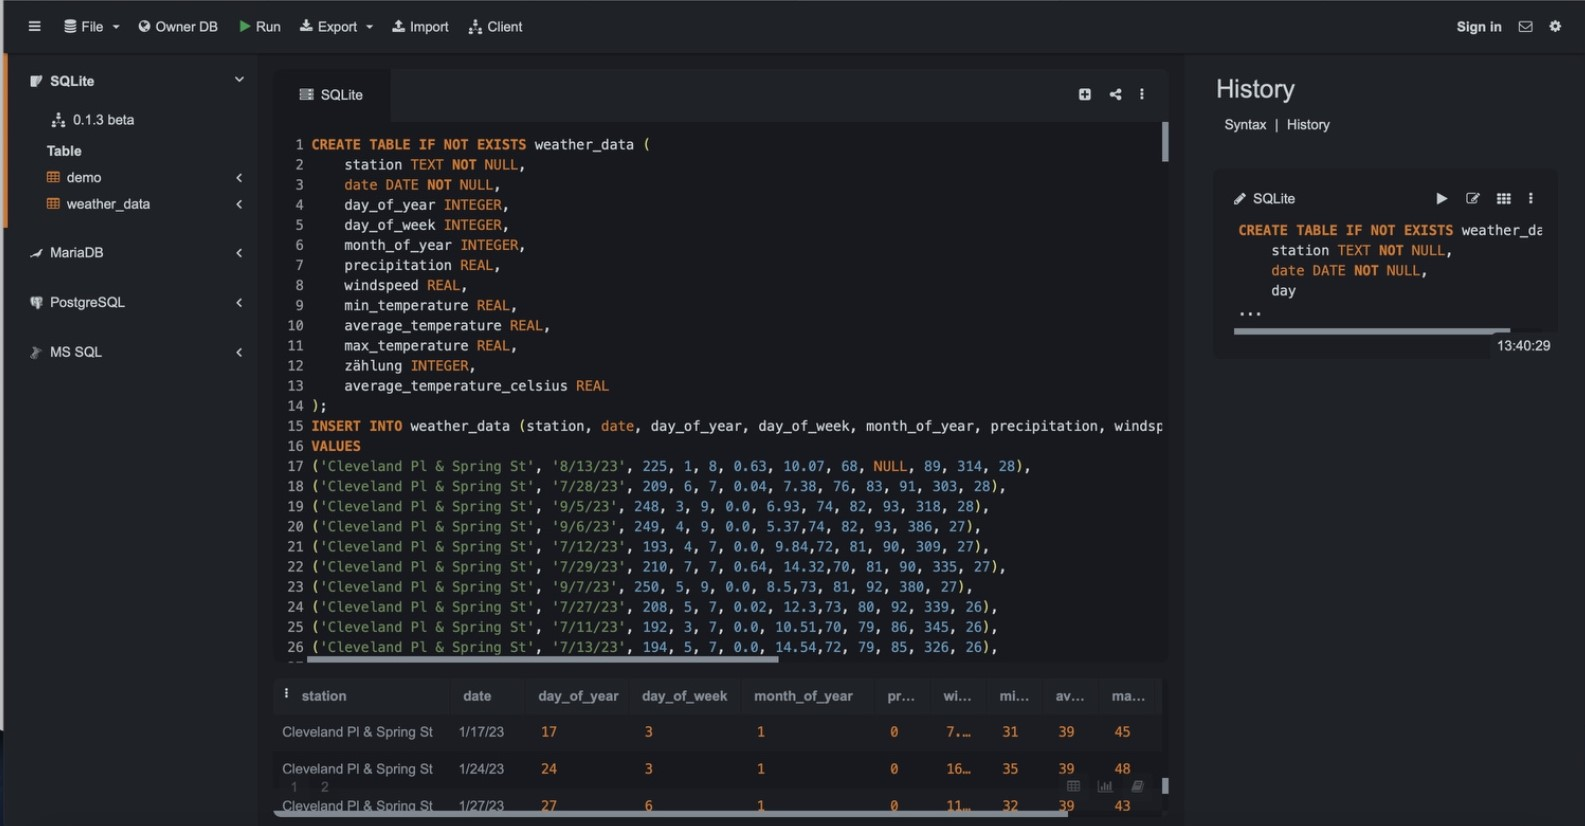
\includegraphics[width=0.5\linewidth]{Bild1.jpeg}
    \caption{}
    \label{Abb1}
\end{figure}

\begin{figure}
    \centering
    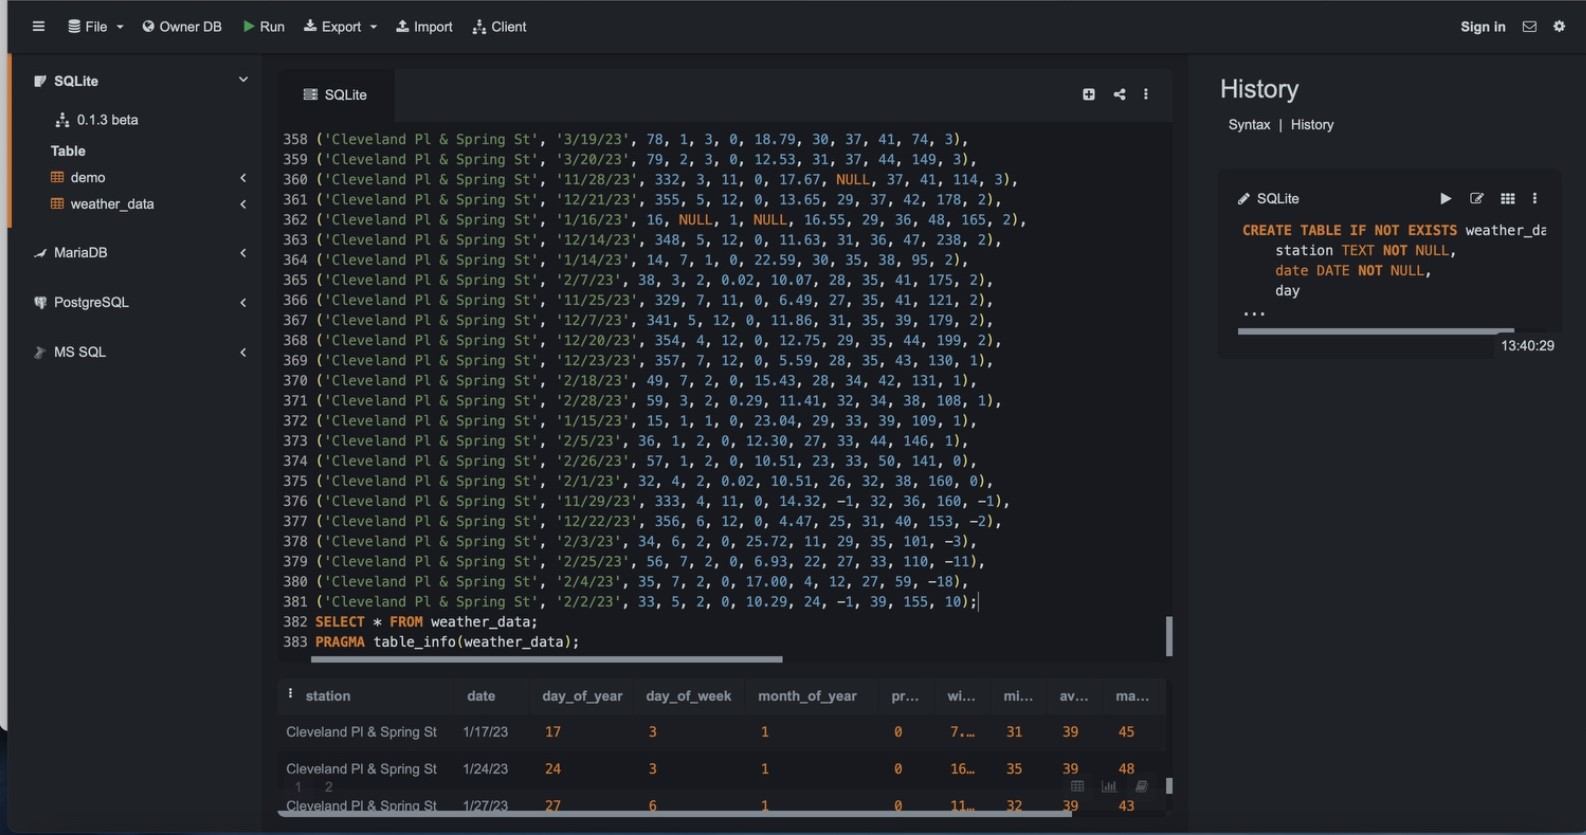
\includegraphics[width=0.5\linewidth]{Bild2.jpeg}
    \caption{}
    \label{Abb2}
\end{figure}

\begin{figure}
    \centering
    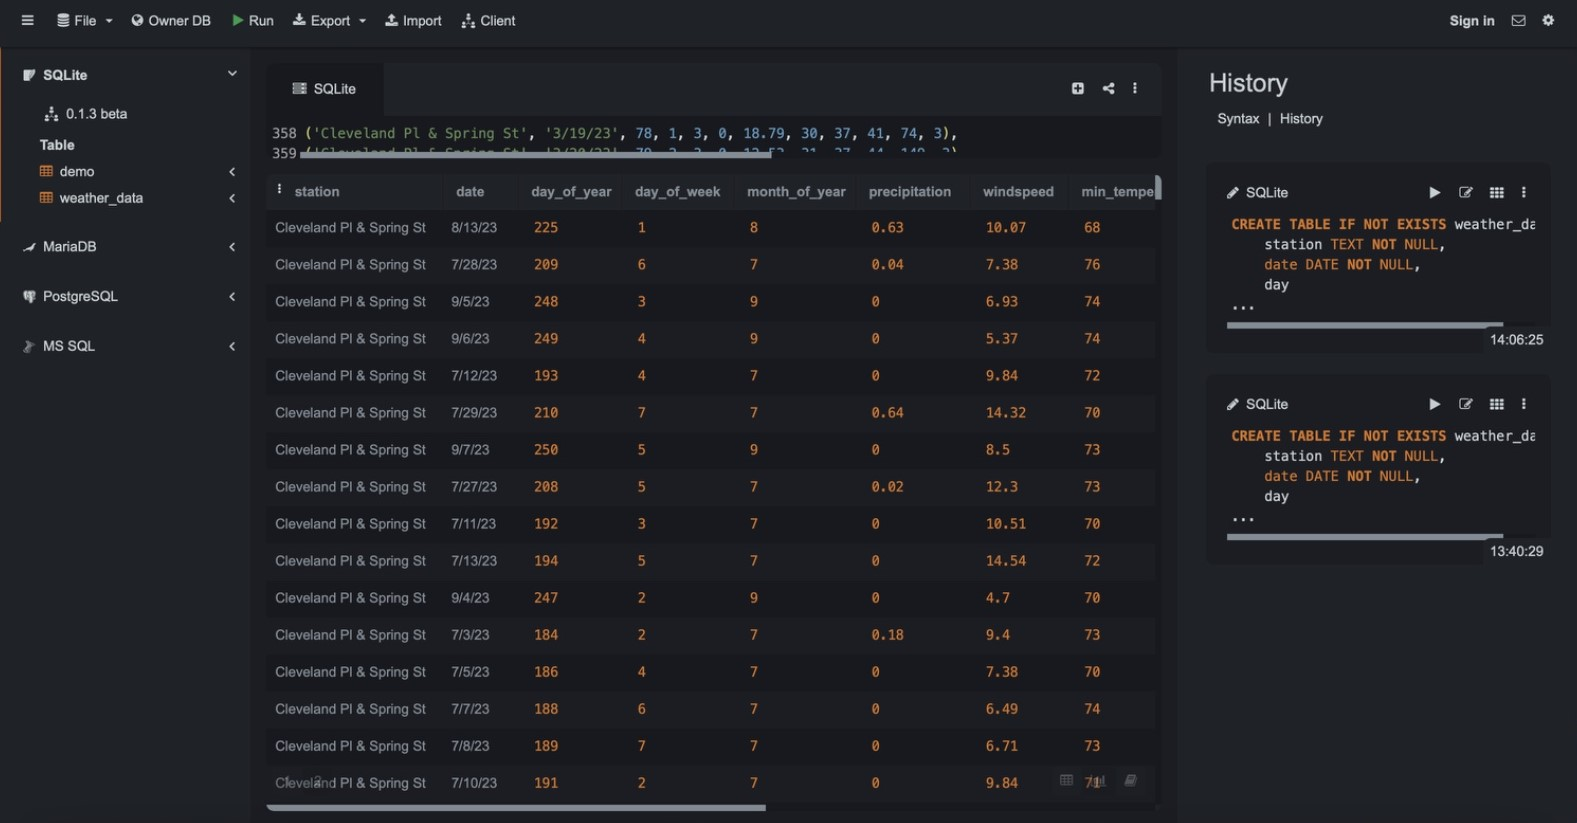
\includegraphics[width=0.5\linewidth]{Bild3.jpeg}
    \caption{}
    \label{Abb3}
\end{figure}

\begin{figure}
    \centering
    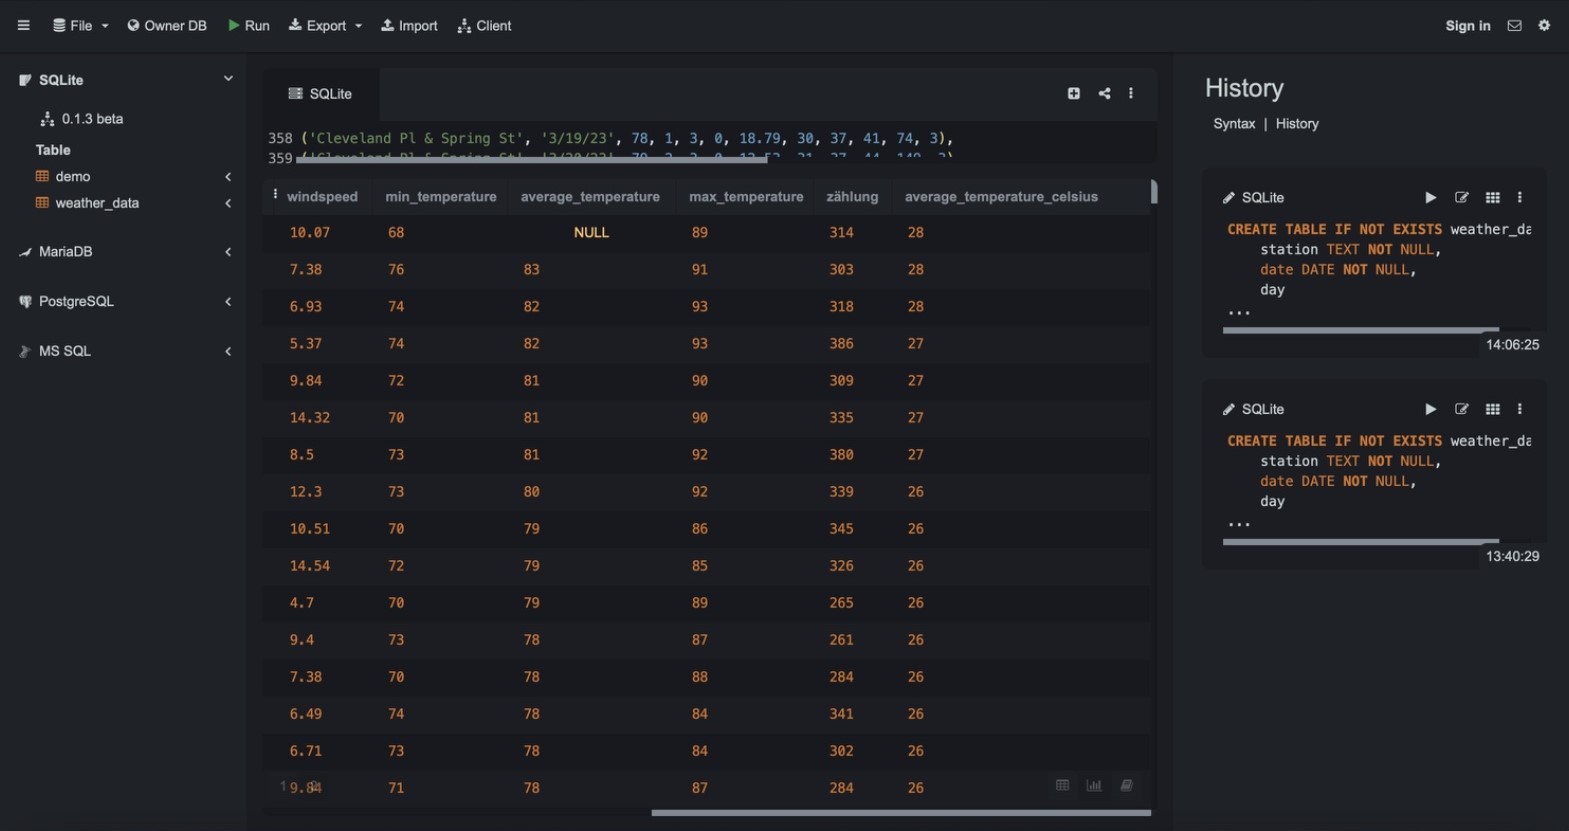
\includegraphics[width=0.5\linewidth]{Bild4.jpeg}
    \caption{}
    \label{Abb4}
\end{figure}

\newpage
\renewcommand{\refname}{Literatur}
\addcontentsline{toc}{section}{Literatur}
\begin{thebibliography}{9}
    \bibitem{klenke2013}
    Achim Klenke,
    \textit{Wahrscheinlichkeitstheorie.},
    Springer, 3. edition, 
    2013.
    \bibitem{overleaf intro}
\href{https://de.overleaf.com/learn/latex/Hyperlinks}{Overleaf Hyperlinks erzeugen}
\end{thebibliography}














\end{document}
